\documentclass[../Article_Model_Parameters.tex]{subfiles}
\graphicspath{{\subfix{../Figures/}}}
\begin{document}
		
	For the sake of clarity of the process model, different colors have been used in the equations to indicate: 
	{\color{red}control variables},
	{\color{blue}state variables},
	{\color{orange}variables} and
	{\color{magenta}parameters}.
	
	\subsubsection{Continuity equation} \label{CH: Continuity}
	The details of derivation can be found in the appendix \ref{CH: Gouverning equations}. The continuity equation for the fluid phase is given by equation \ref{EQ: CompressibleEuler_1}. If $A_f$ is specified to be a function of void fraction $A_f = A\varepsilon(z)$, where $\varepsilon$ is void fraction of the bed and $A$ is the cross-section of the empty extractor. The continuity equation become
	
	{\footnotesize
		\begin{equation*}
			\cfrac{\partial \left( \rho_f \varepsilon \right)}{\partial t} + \cfrac{\partial \left( \rho_f v \varepsilon \right)}{\partial z} = 0
		\end{equation*}
	}
	
	Assuming that the mass flow-rate is constant in time, the temporal derivative become zero and the spacial derivative can be integrated along $z$.
	
	{\footnotesize
		\begin{equation}
			\int \cfrac{\partial \left( \rho_f v \varepsilon \right)}{\partial z} dz = 0 \rightarrow F=\rho_f v \varepsilon
		\end{equation}
	}

	where $F$ is a constant obtained from the integration and it is understood as the mass flux per unit area which is assumed to be constant along $z$. $F$ can treated as a control variable, which can change in time but it is constant in space. Such a assumption allows to find the velocity profile which satisfy the mass continuity based on $F, \varepsilon$ and $\rho_f$. The fluid density $\rho_f$ density is connected through equation of state with thermodynamical pressure, which is assumed to be constant along $z$ (due to the low-Mach number) and temperature \todo{Elaborate, the pressure is know (a control variable) and temperature can be found from energy equation}. The variation in density might be caused by the accumulation of the fluid \todo{Introduce relation between accumulation, pressure and energy equation} in the system (which happen instantaneously along $z$) or by temperature change. To simplify the dynamic of the system, it is assumed that $F=F(t)$ is a control variable and affects the whole system instantaneously.
	
	\subsubsection{Mass balance for the fluid phase} \label{CH: Mass_balance_fluid}
	
	The detail derivation of the mass balance equation for the fluid phase can be found in the appendix (\ref{CH: Gouverning equations}). The movement of the mobile pseudo-homogeneous phase (equation \ref{Model_fluid}) is considered only in the axial direction. The properties of the system in the radial direction are assumed to be uniform. In addition, it is considered that the boundary layer adjacent to the inner wall of the extractor does not exist. Therefore, the velocity profile is constant across any cross-section of the extractor perpendicular to the axial direction. As a result, the plug flow model \todo{Double check if we can call it a plug flow} can be introduced. The particle size distribution and the void fraction of the solid phase cab change along an extractor but they remain constant in time. Moreover, the thermodynamic pressure is considered to be constant along the device, as discussed above. The amount of solute in the solvent is considered negligible. Therefore, the fluid phase can be described as pseudo-homogenous, and its properties are assumed to be the same as the solvent. The mass balance for the fluid phase consists of convection, diffusion, and kinetic terms.
	
	%The process model consists of three partial differential equations: two mass balance equations relative to the concentration of solute in the fixed solid phase and the mobile fluid phase, and the heat balance equation relative to the temperature of the fluid phase.
	
	{\footnotesize
		\begin{align} 
			\label{Model_fluid}
			\cfrac{\partial {\color{blue}c_f}(t,z)}{\partial t} &	=  \underbrace{- \cfrac{u_s}{\varepsilon} \cfrac{\partial {\color{blue}c_f}(t,z)}{\partial {\color{blue}z}}}_{\text{Convective term}} - \underbrace{ \cfrac{ {\color{blue}c_f}(t,z) }{\varepsilon} \cfrac{\partial {\color{blue}u}(t,z)}{\partial {\color{blue}z}}}_{\text{Convective term}} \nonumber \\
			&+ \underbrace{ \cfrac{ {\color{orange}D^M_e} }{\varepsilon} \left[{\color{blue}T}(t,z),{\color{red}P}(t),{\color{red}F}(t)\right] \cfrac{\partial^2 {\color{blue}c_f}(t,z)}{\partial {\color{blue}z^2}} }_{\text{Diffusive term}} 
			+ \underbrace{ \cfrac{1-{\color{magenta}\varepsilon}}{{\color{magenta}\varepsilon}} {\color{blue}r_e}(t,z) }_{\text{Kinetic term}}
	\end{align} }
	
	where ${\color{blue}c_f}(t,z), {\color{blue}c_s}(t,z), {\color{blue}T}(t,z)$ correspond to concentration of solute in the fluid phase, concentration of solute in the solid phase and the temperature, respectively. ${\color{blue}r_e}(t,z)$ is a mass transfer kinetic term. ${\color{red}F}(t)$ is the mass flow rate, ${\color{red}P}(t)$ is the pressure, ${\color{magenta}\epsilon}$ is the void fraction of the bed, ${\color{orange}\rho}({\color{blue}T}(t,z),{\color{red}P}(t))$ is the fluid's density, ${\color{magenta}\rho_s}$ is the solids density, ${\color{orange}D^M_e}({\color{blue}T}(t,z),{\color{red}P}(t),{\color{red}F}(t))$ is the axial mass diffusion coefficient and $u$ is the superficial velocity. \todo{Remove symbols which have been introduced before}
	
	\subsubsection{Mass balance for the solid phase} \label{Mass_balance_solid}
	
	Considering the solid phase to be fixed, the convection and diffusion terms in the corresponding mass balance (equation \ref{Model_solid}) are both assumed to be negligible or absent. Therefore, the only term present in this equation is the kinetic term (defined as presented in equation \ref{Model_kinetic_basic}), which links solid and fluid phases. A single pseudo-component is used to represent the extract collectively. 
	
	{\footnotesize
		\begin{equation} 
			\label{Model_solid}
			%		{\scriptsize\begin{align*}
					\cfrac{\partial {\color{blue}c_s}(t,z)}{\partial t} = \underbrace{ {\color{blue}r_e}(t,z) }_{\text{Kinetics}}
			\end{equation} }
			
	\subsubsection{Kinetic term} \label{CH: Kinetic}
	
	The kinetic term is based on two-film theory and follow work of \citet{Reverchon1996}. The mass transfer kinetic (equation \ref{Model_kinetic_basic}) consists of the overall diffusion coefficient and the concentration gradient, which acts as a driving force for the process.
	
	As the solvent flows through the bed, the $CO_2$ molecules diffuse into the pores and adsorb on the particle surface to for an external fluid film around the solid particles through the solvent–solid matrix interactions. Assuming that the mean free path of the molecule is much smaller than the pore diameter, the effect of Knudsen diffusion is small and can be neglected. The dissolved solute diffuses from the particle's core through the solid-fluid interface, the pore, and the film into the bulk. The graphical representation of the mass transfer mechanism is shown in Figure \ref{fig: SFE_Mechanism}. The mean solute concentration in the solid phase is denoted as ${\color{blue}c_s}$. At the solid-fluid interface, the equilibrium concentrations are given as ${\color{blue}c_s^*}$ and ${\color{blue}c_P^*}$, respectively for solid and fluid phases. The concentration of the solutes in the fluid phase in the centre of the pore is denoted as ${\color{blue}c_{P}}$. As the solute diffuses through the pore, its concentration changes and reaches ${\color{blue}c_{Pf}}$ at the opening of the pore. The solute diffuses through the film around the particle and reaches a concentration in the bulk ${\color{blue}c_f}$. It can be assumed that the two-film theory describes the solid-fluid interface inside the pore. The overall mass transfer coefficient can be introduced if the relation between the solute concentration in one phase and its equilibrium concentration is known.
			
		\begin{figure}[h!]
			\centering
			%	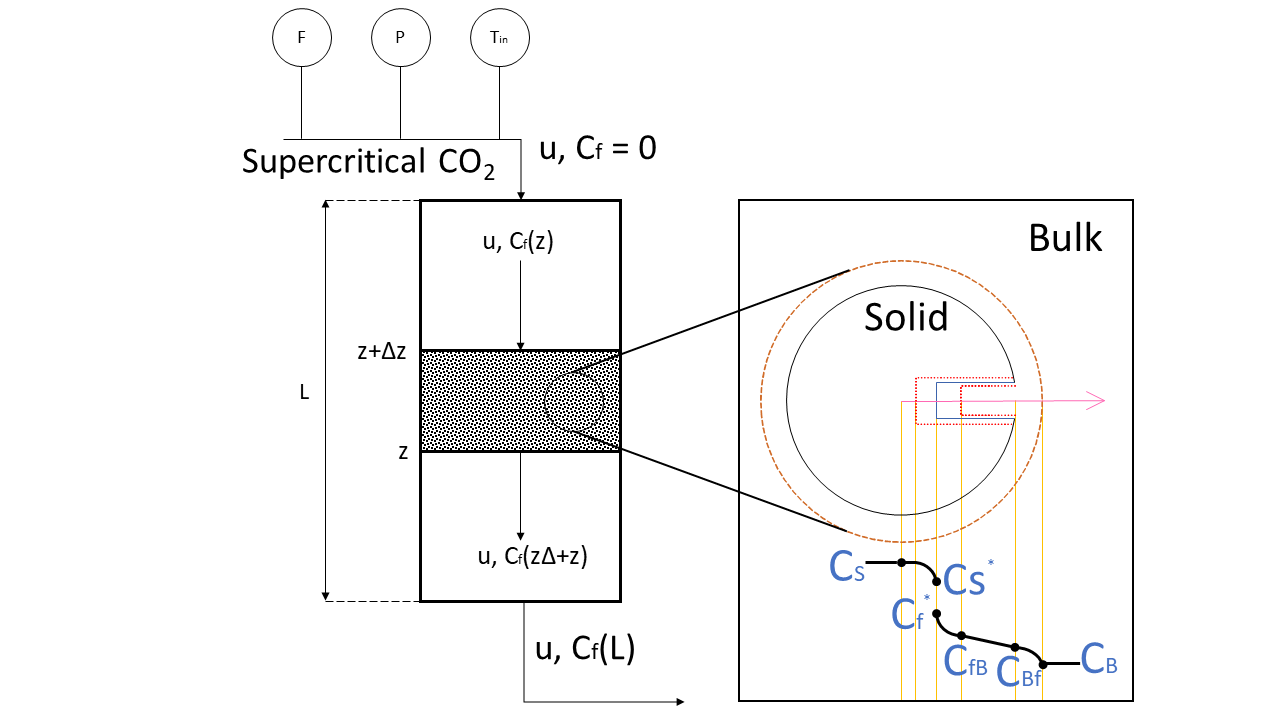
\includegraphics[trim  = 6cm 0cm 3cm 0cm,clip,width=\linewidth]{Figures/SFE_draft.png}
			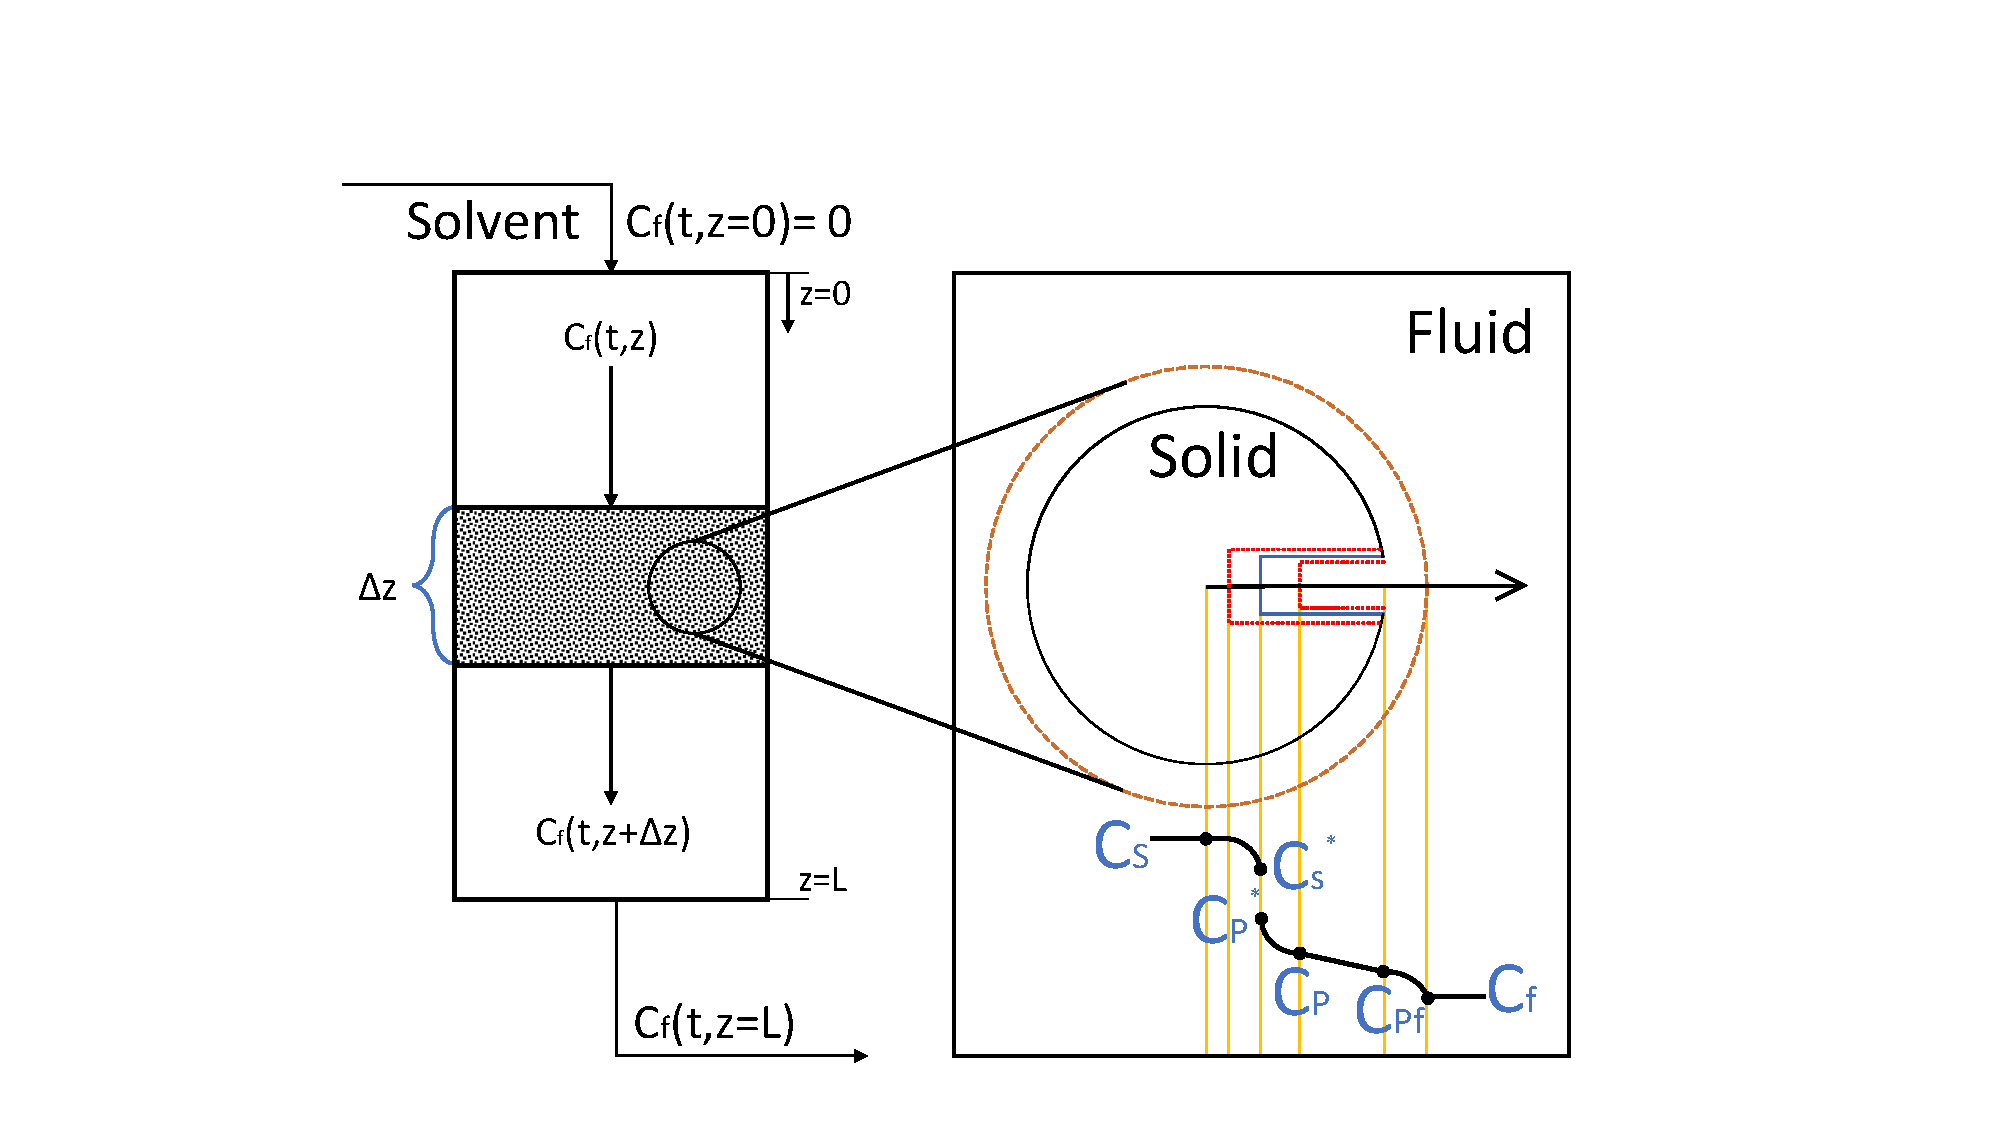
\includegraphics[trim = 5.8cm 1.1cm 6cm 3cm,clip,width=\columnwidth]{Figures/SFE_draft.pdf}	
			\caption{The extraction mechanism}
			\label{fig: SFE_Mechanism}
		\end{figure}
			
		\citet{Bulley1984} suggest a process where the driving force for extraction is given by the difference between concentration of the solute in the bulk, ${\color{blue}c_f}$, and in the centre of the pore, ${\color{blue}c_P^*}$. The concentration ${\color{blue}c_P^*}$ is in equilibrium with ${\color{blue}c_s}$ according to an equilibrium relationship. The rate of extraction is thus ${\color{blue}r_\text{e}}\left({\color{blue}c_f} - {\color{blue}c^*_P}({\color{blue}c_s})\right)$. 
			
		On the other hand, \citet{Reverchon1996} proposes a driving force given by the difference between ${\color{blue}c_s}$ and ${\color{blue}c_P^*}$. ${\color{blue}c_P^*}$ is determined by an equilibrium relationship with ${\color{blue}c_f}$ and the extraction rate is ${\color{blue}r_\text{e}}\left({\color{blue}c_s} - {\color{blue}c^*_P}({\color{blue}c_f})\right)$ or more precisely
			
			{\footnotesize
				\begin{equation} \label{Model_kinetic_basic}
					{\color{blue}r_e}(t,z) = \cfrac{{\color{orange}D_i}({\color{blue}T}(t,z), {\color{red}P}(t))}{{\color{magenta} \mu l^2} }\left({\color{blue}c_s}(t,z) - {\color{blue}c_P^*}(t,z) \right)
			\end{equation} }
			
		where ${\color{magenta}\mu}$ is sphericity, ${\color{magenta}l}$ a characteristic dimension of particles and can be defined as ${\color{magenta}l} = {\color{magenta}r}/3$, ${\color{magenta}r}$ is the mean particle radius, ${\color{magenta}\rho_s}$ is the solid density, ${\color{orange}D_i}({\color{blue}T}(t,z))$ corresponds to the overall diffusion coefficient and ${\color{blue}c_P^*}(t,z)$ is a concentration at the solid-fluid interface (which according to the internal resistance model is supposed to be at equilibrium with the fluid phase). 
			
		According to \citet{Bulley1984}, a linear equilibrium relationship (equation  \ref{Linear_equilibirum}) can be used to find an equilibrium concentration of the solute in the fluid phase ${\color{blue}c_f^*}(t,z)$ is based on concentration of the solute in the solid phase ${\color{blue}c_s}(t,z)$ 
			
			{\footnotesize
				\begin{align} \label{Linear_equilibirum}
					{\color{blue}c}(t,z) &= {\color{orange}k_p}({\color{blue}T}(t,z),{\color{red}P}(t)) \allowbreak {\color{blue}q^*}(t,z)
			\end{align} }
			
			The volumetric partition coefficient ${\color{orange}k_p}({\color{blue}T}(t,z),{\color{red}P}(t))$ behaves as an equilibrium constant between the solute concentration in one phase and the corresponding equilibrium concentration at the solid-fluid interphase. According to \citet{Spiro2007}, the term ${\color{orange}k_p}({\color{blue}T}(t,z),{\color{red}P}(t))$ can be expressed as the function of mass partition factor ${\color{orange}k_m}({\color{blue}T}(t,z))$.
			
			{\footnotesize
				\begin{align}
					{\color{orange}k_m}({\color{blue}T}(t,z)) = \cfrac{{\color{orange}k_p}({\color{blue}T}(t,z),{\color{red}P}(t)) {\color{magenta}\rho_s}}{{\color{orange}\rho}({\color{blue}T}(t,z),{\color{red}P}(t))}
			\end{align} }
			
			Equation \ref{Model_kinetic_no_sat} represents of the kinetic term according to \citet{Reverchon1996}
			
			{\footnotesize
				\begin{equation}
					\label{Model_kinetic_no_sat}
					{\color{blue}r_e}(t,z) = -\cfrac{{\color{orange}D_i}({\color{blue}T}(t,z), {\color{red}P}(t))}{{\color{magenta} \mu l^2} }\left({\color{blue}c_s}(t,z) - \cfrac{{\color{magenta}\rho_s}}{{\color{orange}k_m}({\color{blue}T}(t,z)){\color{orange}\rho}({\color{blue}T}(t,z),{\color{red}P}(t))}  {\color{blue}c_f}(t,z) \right)
			\end{equation} }

        The above model does not take into account the saturation of fluid, which can be introduced by multiplying the gradient by a function $\gamma(c_f)$ (equation \ref{EQ: C_sat_function}). $\gamma(c_f)$ describe the reverse logistic function, which is equal to unity below the $c_{sat}$, the saturation concentration, and equal to zero, above the $c_{sat}$. The $\gamma(c_f)$ for $c_{sat}=5$ is shown on figure \ref{fig: Gamma_function}.

        {\footnotesize
            \begin{equation}
                \gamma(c_f) = \cfrac{1}{1+\exp ( -k_{sat} \left( c_f - c_{sat} \right) ) }
                \label{EQ: C_sat_function}
            \end{equation}
        }

        where $k_{sat}$ is the growth rate, and it is defined as $k_{sat} = 2c_{sat}$\todo{Explain why the growth rate is defined as it is}.
        
        \begin{figure}[h!]
        	\centering
        	\begin{tikzpicture}
        		
        		\begin{axis}[
        			legend style={draw=none},
        			xmin = 0, xmax = 10,
        			ymin = -0.5, ymax = 1.5,
        			xlabel = {$c_f[kg/m^3]$},
        			ylabel = {$\Gamma(c_f)[-]$}]
        			\addplot[
        			domain = 0:10,
        			samples = 100,
        			smooth,
        			thick,
        			blue,
        			] { 1 / (1 + exp( 2*5 .* ( x - 5 ) ) ) };
        			\addplot[thick, samples=50, dashed, domain=0:1.5, black] coordinates {(5,-0.5)(5,1.5)};
        			
        			\addlegendentry{$\gamma(c_f)$}
        			\addlegendentry{$c_{sat}$}
        		\end{axis}
        	        		
        	\end{tikzpicture}
        \caption{$\gamma(c_f)$ function under assumption of $c_{sat}=5 [kg/m^3]$}
        \label{fig: Gamma_function}
        \end{figure}
        

        The final form of the extraction kinetic equation is given by equation \ref{Model_kinetic}.

        {\footnotesize
			\begin{equation}
				\label{Model_kinetic}
				{\color{blue}r_e}(t,z) = -\cfrac{{\color{orange}D_i}({\color{blue}T}(t,z), {\color{red}P}(t))}{{\color{magenta} \mu l^2} } \gamma(c_f) \left({\color{blue}c_s}(t,z) - \cfrac{{\color{magenta}\rho_s}}{{\color{orange}k_m}({\color{blue}T}(t,z)){\color{orange}\rho}({\color{blue}T}(t,z),{\color{red}P}(t))}  {\color{blue}c_f}(t,z) \right)
		\end{equation} }
			
		\subsubsection{Heat balance} \label{CH: heat_balance} \todo{I will be back. The energy equation is not given as a in terms of temperature any more.}
		
		 {\color{red}
			The heat balance (equation \ref{Model_heat}) consists of the convective and diffusive terms. It follows the assumption of a pseudo-homogeneous phase, which properties are the mean between fluid and solid phases. We consider no heat loss through the wall, and there is no heat generation in the system. Therefore, the temperature of the extractor can be changed only by manipulating the temperature of the inlet stream %$T_{In}(t)$. 
			
			We assume that at a given section, where the cross-sectional area is $A$, the flow properties are uniform across that section. Hence, although the area of an extractor changes  as a function of a distance along an extractor (e.g. if a fixed fill an extractor partially), $z$, and therefore in reality the flow field is two-dimensional (the flow varies in the two-dimensional space), we make the assumption that the flow properties vary only with $z$; this is tantamount to assuming uniform properties across any given cross section. Such flow is defined as quasi-one-dimensional flow.
			
		}
		
		\sout{The heat balance equation (equation  \ref{Model_heat}) was developed, assuming the existence of a pseudo-homogeneous phase, which properties are the mean between fluid and solid phases (the amount of solute is considered small enough not to affect the overall heat balance). Equation \ref{Model_heat} contains the convection and the diffusion terms. It is considered that there is no heat loss through the wall, and there is no heat generation in the system. The temperature of the extractor can be changed only by increasing the temperature of the inlet stream. The pseudo-homogenous phase is assumed to flow only in the axial direction. The numerator of the factor in front of the convection term of the heat equation contains only the specific heat of the fluid ${\color{orange}C_p}({\color{blue}T}(t,z),{\color{red}P}(t))$ because the solid phase is stationary. Therefore, this factor can be understood as the fraction of the fluid's total heat through convection. On the other hand, the axial heat diffusion is calculated based on the definition of thermal diffusivity for the fluid, as explained in the appendix. }
			
		{\color{blue} The heat balance (equation \ref{Model_heat}), is based on \citet{Srinivasan2012}, and consists of convective and diffusive terms. It follows the assumption of a pseudo-homogeneous phase, which properties are the mean between fluid and solid phases. It is considered that there is no heat loss through the walls, and there is no heat generation in the system. The temperature of the extractor can be changed only by manipulating the temperature of the inlet stream ${\color{red}T_{Inlet}}(t)$.
			}
			
			{\footnotesize
				\begin{equation} \label{Model_heat}
					\begin{split}
						\cfrac{\partial {\color{blue}T}(t,z)}{\partial t} &= 
						\underbrace{ -\cfrac{{\color{red}F}(t) {\color{orange}C_p}({\color{blue}T}(t,z),{\color{red}P}(t))}{{\color{magenta}A} 	[(1-{\color{magenta}\epsilon}){\color{orange}\rho}({\color{blue}T}(t,z),{\color{red}P}(t)) {\color{orange}C_p} ({\color{blue}T}(t,z),{\color{red}P}(t)) + {\color{magenta} \epsilon \rho_s C_{ps} } ]} \cfrac{\partial {\color{blue}T}(t,z)}{\partial {\color{blue}z}}  }_{\text{Convection}} + \\
						& + \underbrace{ {\color{orange}D^T_e}({\color{blue}T}(t,z),{\color{red}P}(t)) \cfrac{\partial^2 {\color{blue}T}(t,z)}{\partial {\color{blue}z^2}} }_{\text{Diffusion}}
					\end{split}
			\end{equation} }
			
		where $ {\color{orange}D^M_e}({\color{blue}T}(t,z),{\color{red}P}(t),{\color{red}F}(t))$ is the axial mass diffusion coefficient, ${\color{orange}C_p}({\color{blue}T}(t,z),{\color{red}P}(t))$ is the fluid's specific heat, ${\color{magenta}C_{ps}}$ is the specific heat of the solid phase, ${\color{orange}D^T_e}({\color{blue}T}(t,z),{\color{red}P}(t),{\color{red}F}(t))$ is the axial heat diffusion coefficient.

        {\color{blue} The heat equation was introduced in the previous chapter. The heat balance describe movement of the internal energy in the system. For real gases it is complicated to write the heat balance in terms of temperature. Alternatively, the temperature can be obtained based on the equation of state if the internal energy and pressure are know. A roootfinder can be used to find a value of temperature, which satisfy the equation of state given values of internal energy and pressure. The temperature needs to be reconstructed from the internal energy in every time-step.
		}
  
		\subsubsection{Extraction yield} \label{CH: Yield} \todo{Give reference for measurement function}
			
		The efficiency of the process (the yield) is calculated according to equations \ref{Model_measurment_1} to \ref{Model_measurment_2}, which evaluate the mass of solute at the exit of the extraction unit and sums it. The integral form of the measurement equation can be transformed into the differential form, and augmented with model equations to be solved simultaneously.
			
		{\footnotesize
			\begin{align} 
				\label{Model_measurment_1}
%				y(t) \left[ kg \right] &= \int_{t_0}^{t_f} Q(t,z) \left[ \cfrac{m^3}{s} \right] c_f(t,z) \biggr\rvert_{z=L} \left[ \cfrac{kg}{m^3} \right] dt \left[ s \right] \\
				y(t) \left[ kg \right] &= \int_{t_0}^{t_f} \cfrac{F(t)}{\rho(t,z)} \left[ \cfrac{kg}{s} \left( \cfrac{kg}{m^3} \right)^{-1} \right] c_f(t,z) \biggr\rvert_{z=L} \left[ \cfrac{kg}{m^3} \right] dt \left[ s \right] 	\\
%				\cfrac{dy}{dt} \left[ \cfrac{kg}{s} \right] &= Q(t,z) \left[ \cfrac{m^3}{s} \right] c_f(t,z) \biggr\rvert_{z=L} \left[ \cfrac{kg}{m^3} \right]  \\
				\cfrac{dy}{dt} \left[ \cfrac{kg}{s} \right] &= \cfrac{F(t)}{\rho(t,z)} \left[ \cfrac{kg}{s} \left( \cfrac{kg}{m^3} \right)^{-1} \right] c_f(t,z) \biggr\rvert_{z=L} \left[ \cfrac{kg}{m^3} \right]
                \label{Model_measurment_2}
		\end{align}	}
			
		\iffalse	
			
		\subsubsection{State-space representation} \label{CH: State_space}
		It is assumed that the solvent is free of solute at the entrance of the extractor and that all the solid particles have the same initial solute content ${\color{magenta}q_0}$. Moreover, it is considered that the initial temperature of the extractor in every place is equal to ${\color{magenta}T_0}$. Therefore, the initial conditions employed in the simulation are:
			
		{\footnotesize
			\begin{subequations}
				\begin{align*}
					{\color{blue}c}(t = 0, z) &= 0   \\
					{\color{blue}q}(t = 0, z) &= {\color{magenta}q_0} \\
					{\color{blue}T}(t = 0, z) &= {\color{magenta}T_0}
				\end{align*}
		\end{subequations} }
			
		The process model can be written in a general form:
			
		{\footnotesize
			\begin{align}
				\begin{bmatrix}
					\cfrac{\partial {\color{blue}c}(t,z)}{\partial t}\\
					\cfrac{\partial {\color{blue}q}(t,z)}{\partial t}\\
					\cfrac{\partial {\color{blue}T}(t,z)}{\partial t} 
				\end{bmatrix}
				& =
				\begin{bmatrix}
					{\color{blue}\phi_1} \left( {\color{blue}c}(t,z),{\color{blue}q}(t,z),{\color{blue}T}(t,z); {\color{magenta}\theta} \right)\\
					{\color{blue}\phi_2} \left( {\color{blue}c}(t,z),{\color{blue}q}(t,z),{\color{blue}T}(t,z); {\color{magenta}\theta} \right)\\
					{\color{blue}\phi_3} \left( {\color{blue}c}(t,z),{\color{blue}q}(t,z),{\color{blue}T}(t,z); {\color{magenta}\theta} \right)
				\end{bmatrix} = {\color{blue}\phi} \left( t,z; {\color{magenta}\theta} \right) = \cfrac{\partial {\color{blue}\chi}(t,z)}{\partial t}
		\end{align} }
			
		where ${\color{magenta}\theta}$ is a set of parameters present in the model, ${\color{blue}\phi}$ is a set of functions that correspond to state equations of the model, and ${\color{blue}\chi}$ is the state-space model.
		
		The method of lines is used to transform the process model equations into a set of ODEs denoted as ${\color{blue}G}({\color{blue}x}(t);{\color{magenta}p})$. The partial derivatives in $z$-direction are computed using a first-order and second-order finite difference approximation. The backward finite difference is used to approximate first-order derivative, while the central difference scheme is used to approximate second-order derivative. The length of the fixed bed is divided into $N_z$ equally distributed points in $z$-direction. Each function ${\color{blue}\phi_i}$ is transformed to a corresponding set of $N_z$ discretized equations denoted as ${\color{blue}G}_{i\times N_z+1}$ to ${\color{blue}G}_{(i+1)\times N_z}$, where $i$ corresponds to the process model equation. The state-space model ${\color{blue}\chi}(t,z)$ after the discretization is represented by $\dot{{\color{blue}x}}(t)$ (equation  \ref{discretization}).
			
			{\footnotesize
				\begin{align*} \label{discretization}
					\dot{{\color{blue}x}}(t) &= \cfrac{d {\color{blue}x}(t)}{d t} = 
					\begin{bmatrix}
						\cfrac{d {\color{blue}c_{f,1}}(t)}{d t} 	  \\
						\vdots					  \\
						\cfrac{d {\color{blue}c_{f,N_z}}(t)}{d t} \\
						\\ \hline \\
						\cfrac{d {\color{blue}c_{s,1}}(t)}{d t} 	  \\
						\vdots					  \\
						\cfrac{d {\color{blue}c_{s,N_z}}(t)}{d t} \\
						\\ \hline \\
						\cfrac{d {\color{blue}T_1}(t)}{d t} 	  \\
						\vdots 					  \\
						\cfrac{d {\color{blue}T_{N_z}}(t)}{d t}
					\end{bmatrix}
					=
					\underbrace{\begin{bmatrix}
							{\color{blue}G_1} \left( {\color{blue}x}(t),{\color{blue}q}(t),{\color{blue}T}(t); {\color{magenta}p} \right)\\ 
							\vdots\\ 
							{\color{blue}G_{N_z}} \left( {\color{blue}c}(t),{\color{blue}q}(t),{\color{blue}T}(t); {\color{magenta}p} \right)\\ 
							\\ \hline \\ \\
							{\color{blue}G_{N_z+1}} \left( {\color{blue}c}(t),{\color{blue}q}(t),{\color{blue}T}(t); {\color{magenta}p} \right)\\ 
							\vdots\\
							{\color{blue}G_{2N_z}} \left( {\color{blue}c}(t),{\color{blue}q}(t),{\color{blue}T}(t); {\color{magenta}p} \right)\\ 
							\\ \\ \hline \\ 
							{\color{blue}G_{2N_z+1}} \left( {\color{blue}c}(t),{\color{blue}q}(t),{\color{blue}T}(t); {\color{magenta}p} \right) \\
							\vdots\\
							{\color{blue}G_{3N_z}} \left( {\color{blue}c}(t),{\color{blue}q}(t),{\color{blue}T}(t); {\color{magenta}p} \right)
					\end{bmatrix}}_{{\color{blue}G} \left( {\color{blue}x}(t); {\color{magenta}p} \right)} 
			\end{align*} }
			
			where ${\color{blue}x} \in \mathbb{R}^{N_x = 3N_z} $ and ${\color{magenta}p} \in \mathbb{R}^{N_p =  N_{\theta} + N_u } $, $N_{\theta}$ is the number of model parameters, $N_{u}$ is the number of control variables.
			
			{\color{blue} In a state-space sense, the state variables of the system are the local concentrations of solute in the fluid and solid phases ($c(t,z)$ and $q(t,z)$, respectively), and the local temperature of the pseudo-homogeneous phase ($T(t,z)$). The controllable input variables are the mass flow-rate and temperature of the solvent in the feed ($F_\text{in}(t) = F(t)$ and $T_\text{in}(t) = T(t,z=0)$, respectively) and the pressure in the extractor ($P(t,z) = P(t)$). {\color{red}We also assume that extraction yield can be modelled as a function of a known initial mass of solute in the solid phase and it can be measured after the separator ($Y(t)$).} The system is controllable by manipulating the flow-rate and temperature of CO2 in the feed, and the pressure in the extractor. }
			
			\fi
			
\end{document}